\chapter{SVM and kernels: practical aspects and critical view}\label{ch-14}

This slide deck complements
\href{13\%20-\%20Support\%20Vector\%20Machines}{13 - Support Vector
Machines} with a critical view: strengths and weaknesses of SVMs,
examples of results, the crucial role of hyperparameters, some myths to
debunk and the generalisation to \textbf{kernel methods}.

\section{Main features}\label{caratteristiche-principali}

\begin{boxabstract}{Strengths}

\begin{itemize}
\tightlist
\item
  \textbf{Regularisation built into} the optimisation problem (the
  margin).
\item
  \textbf{Approximation of} theoretical \textbf{SRM} (the bound on the
  VC-dim of hyperplanes is minimised by the solution, in the hard
  margin case without kernels).
\item
  \textbf{Convex problem}: training always finds the \textbf{global
  minimum} (unlike neural networks).
\item
  \textbf{Implicit feature transformation} through kernels.
\end{itemize}

\end{boxabstract}

\begin{boxwarning}{Weaknesses}

\begin{itemize}
\tightlist
\item
  One must \textbf{choose the kernel and its parameters}.
\item
  It is a \textbf{batch} algorithm.
\item
  Very large problems used to be computationally intractable: beyond
  about 20,000 examples it was difficult to solve them exactly with
  standard approaches (the kernel matrix is \(N \times N\)). Today there
  are many solutions, including gradient-descent-based ones.
\end{itemize}

\end{boxwarning}

In short, the advantages:

\begin{itemize}
\tightlist
\item
  a \textbf{linear model} (simple, compact) with a bound on complexity
  in terms of the \textbf{margin}, which is optimised directly;
\item
  a rich set of \textbf{non-linear decision functions} in the input
  space through kernels: it is still a linear separation, but in a
  different space, with an \textbf{efficient} treatment of LBE. A rich
  set does not necessarily imply a high VC-dim, which for SVMs depends
  on the margin, the kernel parameters, \(C\), etc.;
\item
  the \textbf{kernel trick} extends to other models: \textbf{kernel
  methods}.
\end{itemize}

\section{Results}\label{risultati}

\subsection{The first famous
application}\label{la-prima-applicazione-famosa}

Handwritten digit recognition (\textbf{MNIST}) was a historic success
case for SVMs: about 0.8\% errors in 1998 with a degree-9 polynomial
SVM, a remarkable result, comparable to LeNet and obtained without
years of architecture development. Interest in SVMs and SLT (whose
studies dated back to the 1960s--70s) grew considerably: an example of
the relevance of applications, or of the importance of good theory for
successful applications.

\subsection{The Gaussian mixture
example}\label{lesempio-della-miscela-di-gaussiane}

Let us go back to the two-class problem (mixture of Gaussians) already
seen with linear models, K-NN and neural networks.

\begin{figure}[htbp]
\centering
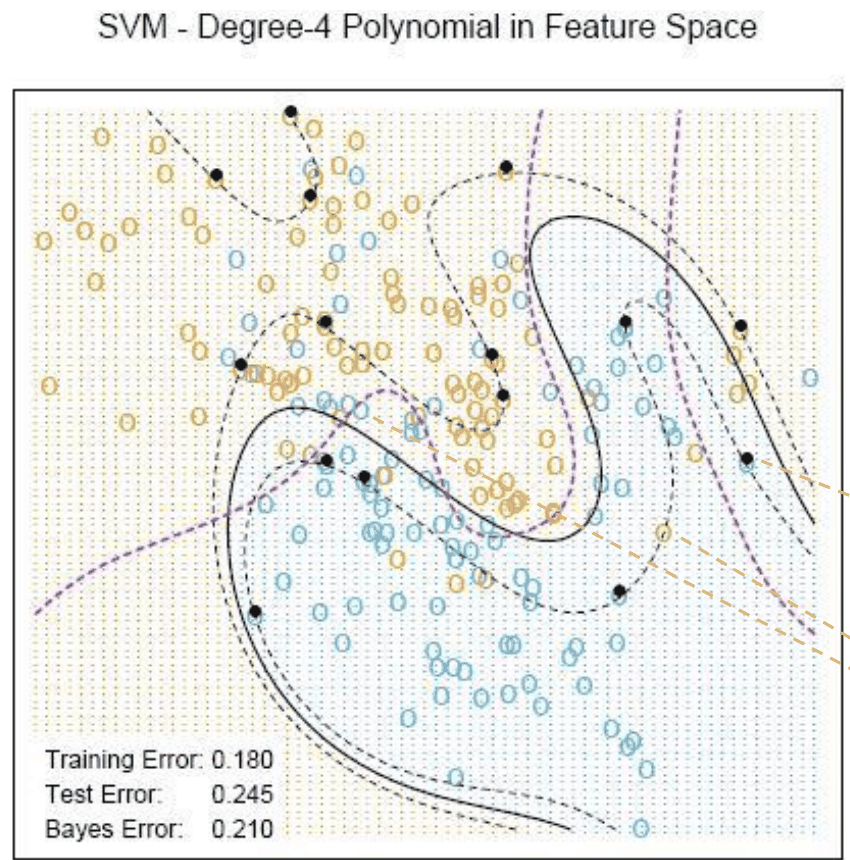
\includegraphics[width=0.51\linewidth,height=0.42\textheight,keepaspectratio]{images/14-svmo_poly.png}
\caption{SVM with a degree-4 polynomial kernel (\(C = 1\)): 42\% of the
data turn out to be support vectors.}
\end{figure}

\begin{figure}[htbp]
\centering
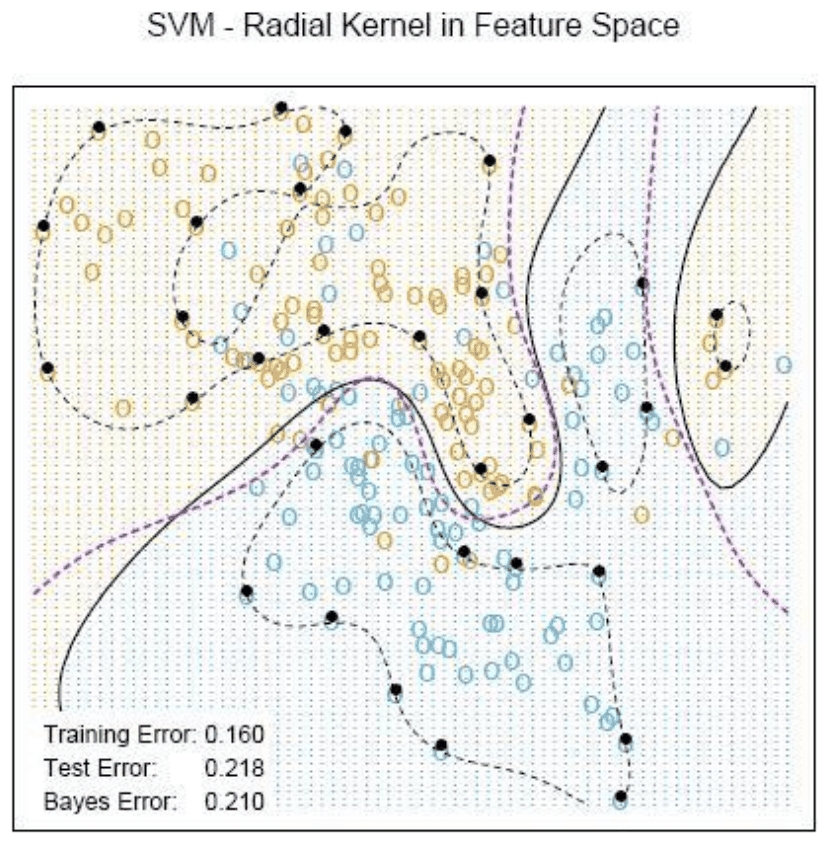
\includegraphics[width=0.51\linewidth,height=0.42\textheight,keepaspectratio]{images/14-svmo_rbf.png}
\caption{SVM with an RBF kernel (\(\gamma = 1/(2\sigma^2) = 1\)): 45\% of
the data are support vectors.}
\end{figure}

Support vectors are the points \textbf{on the margin} (slack = 0) or
\textbf{on the wrong side} of the margin (slack \textgreater{} 0). The
radial kernel gives the best result, as can be expected given that the
data come from Gaussian mixtures. Compare with the neural network with
10 units and weight decay 0.02 (test error 0.223): similar results.

\begin{boxwarning}{Many support vectors}

In theory support vectors are assumed to be few, but \textbf{this is
not always true}: here they are more than 40\% of the data. Sparsity of
the solution is not guaranteed.

\end{boxwarning}

\section{SVMs in practice}\label{le-svm-nella-pratica}

\begin{boxnote}{No guarantee}

\emph{``There is currently no theory that guarantees that a given family
of SVMs will have high accuracy on a given problem''} (Burges, 1998).

\end{boxnote}

The nice properties of hard margin classifiers \textbf{do not extend
directly} to the soft margin and to kernels: the parameter \(C\) and
the kernel can lead to a VC-dim that is even \textbf{infinite}. For
example:

\begin{itemize}
\tightlist
\item
  an SVM with a Gaussian kernel of \textbf{sufficiently small width
  \(\sigma\)} can correctly classify an arbitrarily large number of
  points (like 1-NN, only the support vector closest to \(\mathbf{x}\)
  contributes to the solution): infinite VC-dim, unless regularised;
\item
  conversely, with a \textbf{large} width all support vectors
  contribute and one obtains a sort of ``global average'', with low
  VC-dim.
\end{itemize}

Therefore \textbf{by controlling the kernel width one controls the
VC-dim}.

\subsection{The critical role of
hyperparameters}\label{il-ruolo-critico-degli-iperparametri}

\begin{figure}[htbp]
\centering
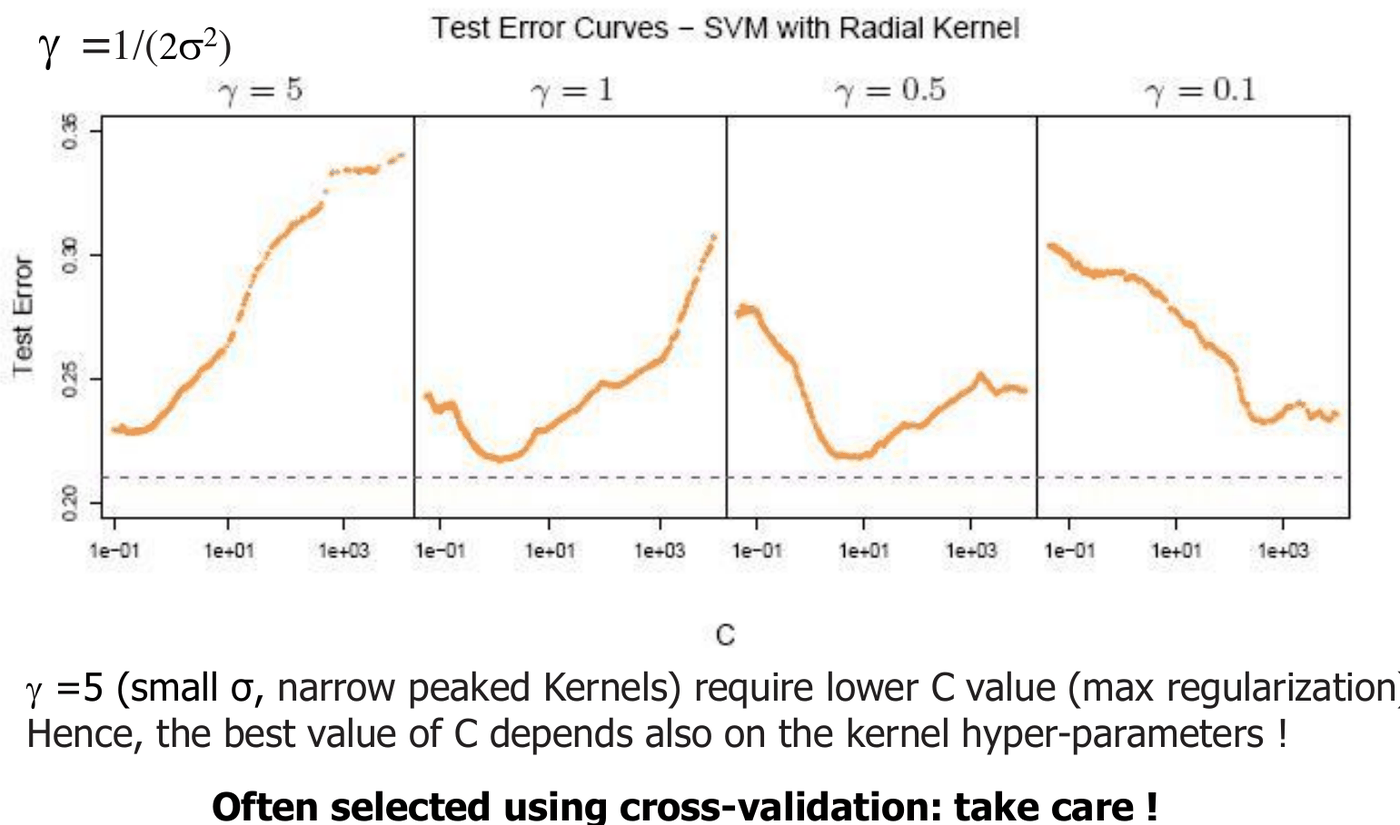
\includegraphics[width=0.86\linewidth,height=0.42\textheight,keepaspectratio]{images/14-svmo_iperparametri.png}
\caption{Test error as a function of \(C\) for different values of
\(\gamma = 1/(2\sigma^2)\).}
\end{figure}

With \(\gamma = 5\) (small \(\sigma\), very narrow kernels) a low \(C\)
(maximum regularisation) is needed; with small \(\gamma\) the optimum
moves towards higher \(C\). \textbf{The best value of \(C\) also
depends on the kernel hyperparameters}: they must be selected
\textbf{together} (grid search), usually with cross-validation,
carefully.

To apply an SVM one must therefore choose the \textbf{type of kernel}
(and its parameters) and the value of \textbf{\(C\)} (and of
\(\varepsilon\) for regression). A rigorous selection would require an
estimate of the complexity (VC-dim); the hyperparameters that affect
complexity are those to be used in model selection. In practice one
performs, once again, a \textbf{careful empirical evaluation}: tuning
the hyperparameters (\(C\), \(\gamma\)\ldots) can introduce
overfitting, hence validation set + test set, or double CV.

Performance: often good, but the comparison with other methods is not
always favourable. Since 2012--2013 \textbf{deep networks} have clearly
beaten the previous records in image and speech recognition.

\subsection{Myths about SVMs}\label{luoghi-comuni-sulle-svm}

\begin{boxquestion}{Exercise: what is wrong?}

\begin{enumerate}
\def\labelenumi{\arabic{enumi}.}
\tightlist
\item
  \emph{``The SVM can be used with the default hyperparameter
  values.''} → No: \(C\) and the kernel parameters are critical and must
  be selected.
\item
  \emph{``I choose the SVM because it does not overfit.''} → No: with
  soft margin and kernels the VC-dim can be very high; overfitting
  depends on \(C\) and on the kernel.
\item
  \emph{``The SVM has no problems with high-dimensional inputs (does
  it solve the curse of dimensionality?).''} → \textbf{No}: the SVM
  handles well the high dimension of the \textbf{feature space}, not of
  the \textbf{input space}. The curse of dimensionality of the input
  remains.
\item
  \emph{``With the SVM the number of units is found automatically.''}
  → The number of support vectors is determined by the solution, but it
  depends on \(C\) and on the kernel, which must be chosen; and it is
  not necessarily small.
\end{enumerate}

\end{boxquestion}

\section{Kernel methods}\label{metodi-kernel}

The \textbf{kernel trick} leads to \textbf{kernel methods}, even
without SVMs: the ``\textbf{kernelisation}'' of traditional approaches.
Whenever a \textbf{dot product} or a \textbf{similarity measure}
appears in a model, it can be replaced with a kernel, making the model
operate in a new implicit high-dimensional space simply by specifying
(and changing) the kernel.

\begin{itemize}
\tightlist
\item
  It is a fixed, high-dimensional \textbf{linear basis expansion}, but
  very \textbf{efficient}.
\item
  The choice of the basis functions is \textbf{modular}: the kernel is
  changed without changing the learning machine.
\item
  It provides a unified theoretical framework for general dot-product
  functions.
\end{itemize}

\subsection{Kernel as a similarity
measure}\label{kernel-come-misura-di-similarituxe0}

The kernel is related to a \textbf{similarity} measure between
\(\mathbf{s}\) and \(\mathbf{t}\); indeed it induces the distance in
the feature space: \[
d_k(\mathbf{s}, \mathbf{t})^2 = k(\mathbf{s}, \mathbf{s}) - 2k(\mathbf{s}, \mathbf{t}) + k(\mathbf{t}, \mathbf{t}) = \|\Phi(\mathbf{s}) - \Phi(\mathbf{t})\|^2.
\] Similar objects (small distance) → high kernel value.

\begin{boxtip}{The idea of kernels}

Focus on representing and processing \textbf{pairwise comparisons} of
objects, rather than on the representation of a single object. In some
domains it is easier to compare two objects than to define an abstract
feature space in which to represent one of them.

\end{boxtip}

An SVM is characterised largely by the choice of the kernel. Compare
with \textbf{neural networks}, where the basis functions \textbf{adapt}
to the data (by learning the weights of the hidden units): in SVMs the
choice of the best kernel for a problem is still a research topic.

(Exercise: rethink the kernel as in distance-based methods, like K-NN.
When is a kernel good? When it groups objects of the same class in the
feature space, reflecting the similarity relevant to the task. When is
it bad? When the similarity it induces has nothing to do with the
task, for example if all objects turn out to be equally similar or
equally different.)

\begin{figure}[htbp]
\centering
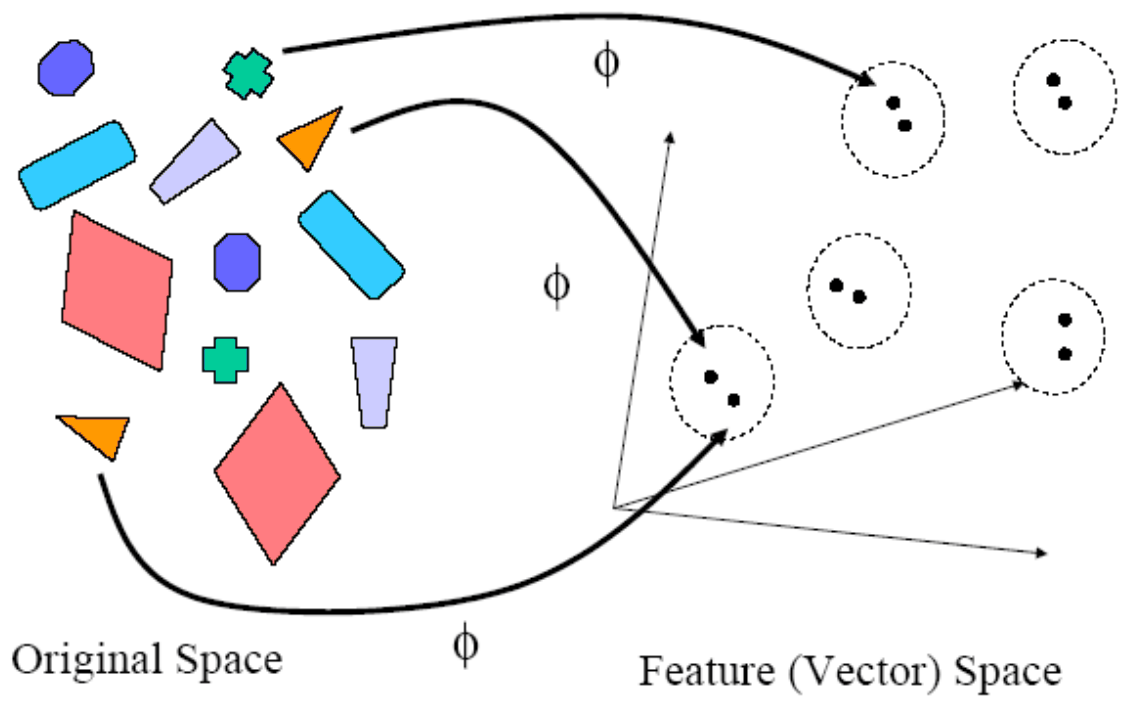
\includegraphics[width=0.63\linewidth,height=0.42\textheight,keepaspectratio]{images/14-svmo_oggetti.png}
\caption{A good kernel for ``objects'': the map \(\phi\) brings similar
objects close together in the feature space.}
\end{figure}

\subsection{Advanced topics}\label{argomenti-avanzati}

\textbf{Designing new kernels} requires choosing a ``good'' function
for the specific domain, and it can be extended to \textbf{generic
objects} as input, not only vectors: kernels for \textbf{strings, trees,
graphs}; ad hoc kernels for the domain and the task (for example
kernels based on \emph{edit distance} for bioinformatics, or on
\emph{suffix trees} for strings in NLP), with attention to algorithmic
efficiency. \textbf{Adaptive kernels} are a research topic.

A conceptual advantage: \textbf{domain knowledge is separated from the
solver}, because it lies entirely in the kernel.

\begin{boxabstract}{Summary}

SVMs combine a linear model, a convex problem with a global minimum,
regularisation via the margin and the power of kernels. But they are
not ``magic'': the choice of kernel and hyperparameters (\(C\),
\(\sigma\), \(\varepsilon\)) is critical and must be made with rigorous
validation; support vectors can be many; they do not solve the curse of
dimensionality of the input space. The kernel trick is a general idea
(kernel methods) that makes it possible to work with similarities
between objects, even structured ones.

\end{boxabstract}

\begin{boxquestion}{Possible exam questions}

\begin{itemize}
\tightlist
\item
  Strengths and weaknesses of SVMs compared to neural networks.
\item
  Why can the VC-dim of an SVM with an RBF kernel be infinite? How is
  it controlled?
\item
  Why must \(C\) and the kernel parameters be selected together?
\item
  Does the SVM solve the curse of dimensionality?
\item
  What are kernel methods? What is the relationship between kernels and
  similarity?
\end{itemize}

\end{boxquestion}
